\section{Kapitel 8}
\subsection{Aufgabenstellung}
Wir sollen ein Klasse schreiben die Nur Gerade zahlen annimmt, andernfalls soll eine Exception
geworfen werden. Zusätzlich kommen noch zwei Methoden in diese Klasse für 
die Multiplikation und Addition.

\subsection{Anforderungsdefinition}
\begin{enumerate}
	\item Erstelle eine Klasse GeradeZahl.
	\item Erstelle eine Methode für die Multiplikation und Addition.
	\item Bei ungeraden Zahlen soll eine Exception geworfen werden.
\end{enumerate}

\subsection{Entwurf}
\begin{center}
	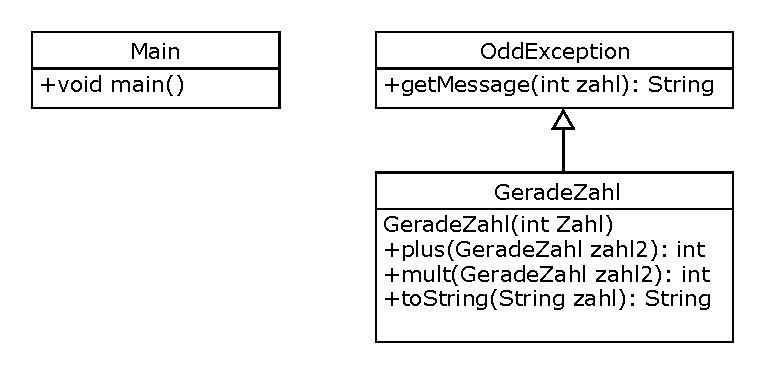
\includegraphics[width=0.99\textwidth]{uml/uml_c8_p1.pdf}
\end{center}

\subsection{Quelltext}
\subsubsection{Main.java}
\lstinputlisting[language = Java , frame = trBL , escapeinside={(*@}{@*)}]{../chapter_08/src/main/java/chapter_08/Main.java}
\subsubsection{GeradeZahl.java}
\lstinputlisting[language = Java , frame = trBL , escapeinside={(*@}{@*)}]{../chapter_08/src/main/java/chapter_08/GeradeZahl.java}
\subsubsection{OddException.java}
\lstinputlisting[language = Java , frame = trBL , escapeinside={(*@}{@*)}]{../chapter_08/src/main/java/chapter_08/OddException.java}

\subsection{Testdokumentation}
Bei einer Ungeraden Zahl wurde eine Exception geworfen und wie erwarte die Zahl
anschließend um eins erhöht.

\subsection{Benutzungshinweise}
Keine Besonderen Benutzungshinweise.
Das Programm muss lediglich nur ausgeführt werden.

\subsection{Anwendungsbeispiel}
Bei einer ungeraden Zahl sollte diese Ausgabe erscheinen.
\begin{lstlisting}[frame = trBL , escapeinside={(*@}{@*)}]
[sebastian@laptop bin]$ java Main
Exception in thread "main" chapter_08.OddException: Error, 21 ist keine Gerade Zahl! Die Zahl wurde um Eins erhöht.
at chapter_08.GeradeZahl.<init>(GeradeZahl.java:14)
at chapter_08.Main.main(Main.java:11)
[sebastian@laptop bin]$ 
\end{lstlisting}
Und bei einer Geraden diese.
\begin{lstlisting}[frame = trBL , escapeinside={(*@}{@*)}]
[sebastian@laptop bin]$ java Main
Zahl 1 = 200
Zahl 2 = 20
Zahl 3 = 600
Zahl 4 = 24
[sebastian@laptop bin]$ 
\end{lstlisting}